\documentclass[14pt]{beamer}
\usepackage{./Estilos/BeamerUVM}
\usepackage{./Estilos/ColoresLatex}
%Sección para el tema de beamer, con el theme, usercolortheme y sección de footers
\usetheme{CambridgeUS}
\usecolortheme{default}
%\useoutertheme{default}
\setbeamercovered{invisible}
% or whatever (possibly just delete it)
\setbeamertemplate{section in toc}[sections numbered]
\setbeamertemplate{subsection in toc}[subsections numbered]
\setbeamertemplate{subsection in toc}{\leavevmode\leftskip=3.2em\rlap{\hskip-2em\inserttocsectionnumber.\inserttocsubsectionnumber}\inserttocsubsection\par}
\setbeamercolor{section in toc}{fg=blue}
\setbeamercolor{subsection in toc}{fg=blue}
\setbeamercolor{frametitle}{fg=blue}
\setbeamertemplate{caption}[numbered]

\setbeamertemplate{footline}
\beamertemplatenavigationsymbolsempty
\setbeamertemplate{headline}{}


\makeatletter
\setbeamercolor{secºtion in foot}{bg=gray!30, fg=black!90!orange}
\setbeamercolor{subsection in foot}{bg=blue!30!yellow, fg=red}
\setbeamercolor{date in foot}{bg=black, fg=white}
\setbeamertemplate{footline}
{
  \leavevmode%
  \hbox{%
  \begin{beamercolorbox}[wd=.333333\paperwidth,ht=2.25ex,dp=1ex,center]{section in foot}%
    \usebeamerfont{section in foot} \insertsection
  \end{beamercolorbox}%
  \begin{beamercolorbox}[wd=.333333\paperwidth,ht=2.25ex,dp=1ex,center]{subsection in foot}%
    \usebeamerfont{subsection in foot}  \insertsubsection
  \end{beamercolorbox}%
  \begin{beamercolorbox}[wd=.333333\paperwidth,ht=2.25ex,dp=1ex,right]{date in head/foot}%
    \usebeamerfont{date in head/foot} \insertshortdate{} \hspace*{2em}
    \insertframenumber{} / \inserttotalframenumber \hspace*{2ex} 
  \end{beamercolorbox}}%
  \vskip0pt%
}






% \usefonttheme{serif}
\usepackage[clock]{ifsym}
\usepackage{pstricks-add}
\DeclareSIUnit\erg{erg}
\DeclareSIUnit[number-unit-product = {\,}]\cal{cal}

\sisetup{per-mode=symbol}
\resetcounteronoverlays{saveenumi}

% Macro para agregar el logo de UVM en cada slide de la presentación

\addtobeamertemplate{frametitle}{}{%
\begin{tikzpicture}[remember picture,overlay]
\coordinate (logo) at ([xshift=-1.5cm,yshift=-0.8cm]current page.north east);
% \fill[devryblue] (logo) circle (.9cm);
% \clip (logo) circle (.75cm);
\node at (logo) {
\includegraphics[width=2.1cm]{Imagenes/logo_UVM.png}};
\end{tikzpicture}}


\title{\Large{Fenómenos térmicos} \\ \normalsize{Física III}}
\date{}

\begin{document}
\maketitle

\section*{Contenido}
\frame[allowframebreaks]{\frametitle{Contenido} \tableofcontents[currentsection, hideallsubsections]}

\section{Dilatación térmica}
\frame[allowframebreaks]{\tableofcontents[currentsection, hideothersubsections]}
\subsection{Definición}

\begin{frame}
\frametitle{¿Por qué se dilatan los cuerpos?}
La mayoría de los materiales se \textocolor{ao}{expanden} cuando su temperatura aumenta, \pause y se \textocolor{byzantine}{contraen} cuando la temperatura disminuye.
\end{frame}
\begin{frame}
\frametitle{¿Por qué se dilatan los cuerpos?}    
Esto ocurre porque al calentarse las moléculas se mueven más rápido y ocupan mayor espacio y esto hace que el cuerpo se expanda, \pause y cuando se enfría, las moléculas se mueven más lento y los materiales se contraen.
\end{frame}
\begin{frame}
\frametitle{¿Qué es la dilatación?}    
Este fenómeno se conoce como \textocolor{awesome}{dilatación}, \pause está estrechamente relacionado con los cambios de temperatura de los cuerpos.
\end{frame}
\begin{frame}
\frametitle{Ejemplos de dilatación térmica}
\vspace*{-0.25cm}
\begin{figure}
    \centering
    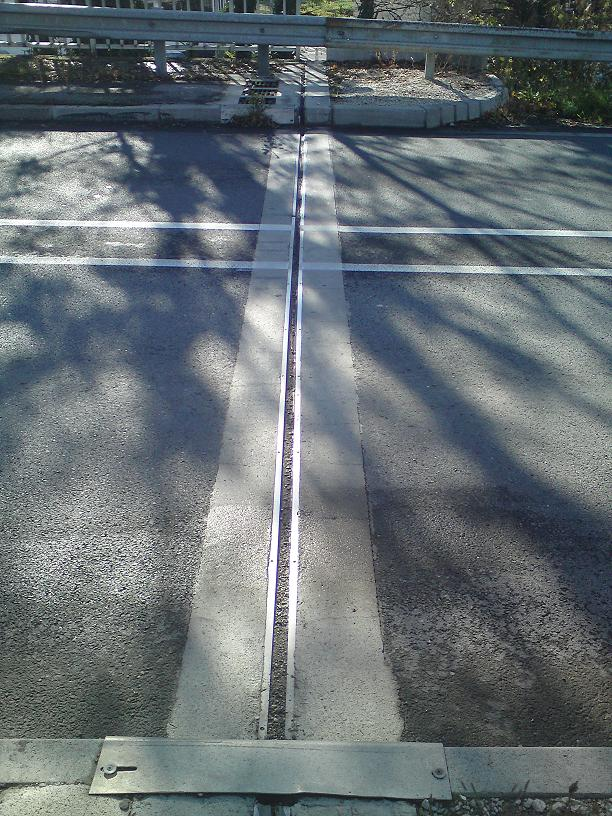
\includegraphics[scale=0.25]{Imagenes/Dilatacion_01.jpg}
\end{figure}
\end{frame}
\begin{frame}
\frametitle{Ejemplos de dilatación térmica}
\vspace*{-0.25cm}
\begin{figure}
    \centering
    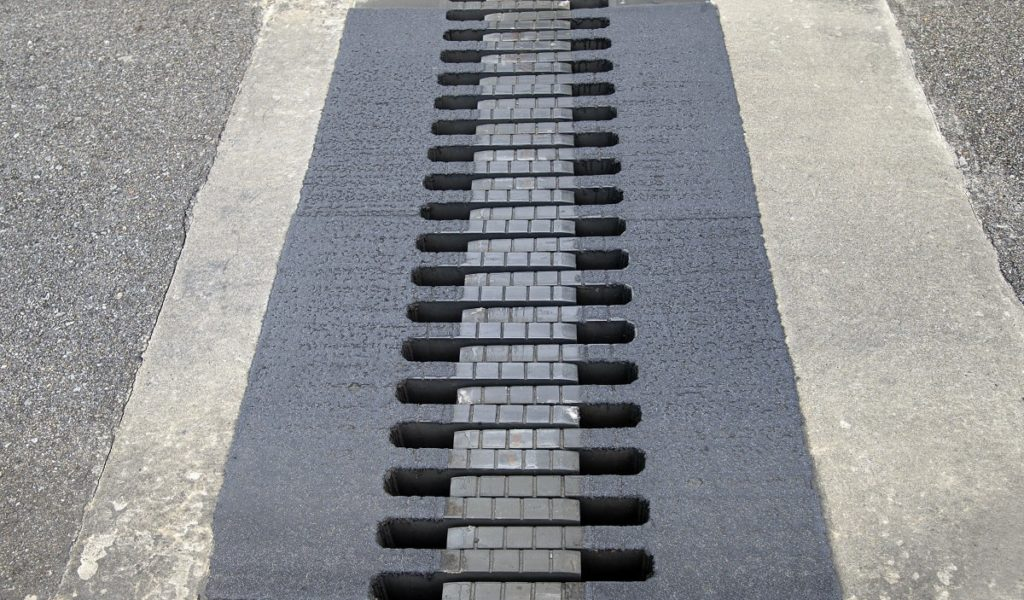
\includegraphics[scale=0.25]{Imagenes/Dilatacion_02.jpg}
\end{figure}
\end{frame}
\begin{frame}
\frametitle{Definición de dilatación}
La \textocolor{bulgarianrose}{dilatación térmica} es el aumento en sus dimensiones que experimenta un cuerpo cuando aumenta la temperatura, permaneciendo la presión constante.
\end{frame}
\begin{frame}
\frametitle{Tipos de dilatación}
Los sólidos se dilatan aumentando su \textocolor{carnelian}{longitud} principalmente, \pause aunque también pueden dilatarse en su \textocolor{coquelicot}{superficie} \pause o \textocolor{cordovan}{volumen}.
\end{frame}
\begin{frame}
\frametitle{Tipos de dilatación}
Al igual que los sólidos, los líquidos y los gases también aumentan o disminuyen su volumen, sin embargo, los gases se dilatan más que los líquidos.
\end{frame}

\subsection{Dilatación lineal}

\begin{frame}
\frametitle{Describiendo la dilatación lineal}
Se ha comprobado experimentalmente que al aumentar la temperatura de una barra, aumenta su \textocolor{cornellred}{longitud} \pause y este aumento es proporcional a su \textocolor{darkcyan}{longitud inicial} \pause y al \textocolor{darkscarlet}{aumento de su temperatura}.
\end{frame}
\begin{frame}
\frametitle{Describiendo la dilatación lineal}
A dicho proceso se le conoce como \textocolor{debianred}{dilatación lineal} y se expresa matemáticamente de la siguiente manera:
\pause
\begin{align*}
\Delta L = \alpha \, L_{i} \, \Delta T
\end{align*}
\end{frame}
\begin{frame}
\frametitle{La dilatación lineal}
\vspace*{-1cm}
\begin{align*}
\Delta L = \alpha \, L_{i} \, \Delta T
\end{align*}
Donde:
\setbeamercolor{item projected}{bg=deeppeach,fg=black}
\setbeamertemplate{enumerate items}{%
\usebeamercolor[bg]{item projected}%
\raisebox{1.5pt}{\colorbox{bg}{\color{fg}\footnotesize\insertenumlabel}}%
}
\begin{enumerate}[<+->]
\item $\Delta L$ es la variación de longitud.
\item $\alpha$ es el coeficiente de proporcionalidad, llamado \textocolor{denim}{coeficiente de dilatación lineal}, es un valor específico para cada material o sustancia.
\seti
\end{enumerate}
\end{frame}
\begin{frame}
\frametitle{Algunos coeficientes}
\begin{table}
    \centering
    \small
    \begin{tabular}{| l | c |} \hline
        Material & $\alpha \, \big[\unit{\degreeCelsius}^{-1} \big]$ \\ \hline
        Concreto & $\numrange{0.7}{1.2d-5}$ \\ \hline
        Plata & \num{2.0d-5} \\ \hline
        Oro & \num{1.5d-5} \\ \hline
        Cobre & \num{1.7d-5} \\ \hline
    \end{tabular}
\end{table}
\end{frame}
% \begin{frame}
% \frametitle{Ejercicio Evaluación Continua}
% Completa la siguiente tabla con los coeficientes de dilatación térmica:
% \pause

% Zinc, Vidrio Pirex, Aluminio, Acetona, Mercurio, Gasolina, Petróleo, Agua a \SI{100}{\degreeCelsius}, Aire, Latón.
% \end{frame}
\begin{frame}
\frametitle{La dilatación lineal}
\vspace*{-1cm}
\begin{align*}
\Delta L = \alpha \, L_{i} \, \Delta T
\end{align*}
Donde:
\setbeamercolor{item projected}{bg=deeppeach,fg=black}
\setbeamertemplate{enumerate items}{%
\usebeamercolor[bg]{item projected}%
\raisebox{1.5pt}{\colorbox{bg}{\color{fg}\footnotesize\insertenumlabel}}%
}
\begin{enumerate}[<+->]
\conti
\item $L_{i}$ es la longitud inicial.
\item $\Delta T$ es la variación de la temperatura.
\end{enumerate}
\end{frame}
\begin{frame}
\frametitle{Consideraciones}
La variación de la longitud $\Delta L$ es la diferencia entre la longitud final, $L_{f}$ y la longitud inicial, $L_{i}$:
\pause
\begin{align*}
\Delta L = L_{f} - L_{i}
\end{align*}
\end{frame}
\begin{frame}
\frametitle{Consideraciones}
La variación de la temperatura $\Delta T$ es la diferencia entre la temperatura final, $T_{f}$ y la temperatura inicial, $T_{i}$:
\pause
\begin{align*}
\Delta T = T_{f} - T_{i}
\end{align*}
\end{frame}
\begin{frame}
\frametitle{La dilatación lineal}
La expresión para la dilatación lineal la podemos expresar como:
\pause
\begin{align*}
L_{f} - L_{i} = \alpha \, L_{i} \, \left( T_{f} - T_{i} \right)
\end{align*}
Expresión que nos será de mucha utilidad.
\end{frame}
\begin{frame}
\frametitle{El coeficiente de dilatación}
Ya que si nos proporcionan la longitud inicial, la final, así como el incremento de la temperatura, podemos calcular el coeficiente de dilatación:
\end{frame}
\begin{frame}
\frametitle{El coeficiente de dilatación}
Tenemos que:
\pause
\begin{eqnarray*}
\begin{aligned}
L_{f} - L_{i} &= \alpha \, L_{i} \, \left( T_{f} - T_{i} \right) \\[0.5em] \pause
\alpha &= \dfrac{L_{f} - L_{i}}{L_{i} \, \left( T_{f} - T_{i} \right)}
\end{aligned}
\end{eqnarray*}
\end{frame}
\begin{frame}
\frametitle{El álgebra en la expresión}
Si nos dan el valor de $\alpha$ y nos piden calcular la longitud final, hacemos el manejo algebraico de la expresión:
\pause
\begin{eqnarray*}
\begin{aligned}
L_{f} - L_{i} &= \alpha \, L_{i} \, \left( T_{f} - T_{i} \right) \\[0.25em] \pause
L_{f} &= \bigg[ \alpha \, L_{i} \, \left( T_{f} - T_{i} \right) \bigg] + L_{i} \\[0.25em] \pause
L_{f} &= L_{i} \bigg[ 1 + \alpha \, \left( T_{f} - T_{i} \right) \bigg]
\end{aligned}
\end{eqnarray*}
\end{frame}
\begin{frame}
\frametitle{Ejercicio 1 - Dilatación lineal}
A una temperatura de \SI{15}{\degreeCelsius} una varilla de hierro tiene una longitud de \SI{5}{\meter}
\\
\bigskip
\pause 
¿Cuál será la longitud al aumentar la temperatura a \SI{25}{\degreeCelsius}?
\end{frame}
\begin{frame}
\frametitle{Resolviendo el ejercicio}
\vspace*{-1cm}
\textocolor{red}{Datos:}
\begin{align*}
\alpha_{Fe} &= \num{11.7d-6} \unit{\degreeCelsius}^{-1} \\
L_{i} &= \SI{5}{\meter} \\
T_{i} &= \SI{15}{\degreeCelsius} \\
T_{f} &= \SI{25}{\degreeCelsius} \\
L_{f} &= \,?
\end{align*}
\end{frame}
\begin{frame}
\frametitle{Resolviendo el ejercicio}
\textocolor{red}{Expresión:}
\begin{align*}
L_{f} &= L_{i} \bigg[ 1 + \alpha \, \left( T_{f} - T_{i} \right) \bigg]
\end{align*}
\end{frame}
\begin{frame}
\frametitle{Resolviendo el ejercicio}
\textocolor{red}{Sustitución:}
\begin{eqnarray*}
\begin{aligned}
L_{f} &= \SI{5}{\meter} \bigg[ 1 + \num{11.7d-6} \, \unit{\degreeCelsius}^{-1} \, \left( \SI{25}{\degreeCelsius} - \SI{15}{\degreeCelsius} \right) \bigg] = \\[0.5em] \pause
L_{f} &= \SI{5.000585}{\meter}
\end{aligned}
\end{eqnarray*}
\end{frame}
\begin{frame}
\frametitle{Dilatación en la varilla}
Ahora ya podemos calcular la dilatación en la varilla:
\pause
\begin{eqnarray*}
\begin{aligned}
L_{f} - L_{i} &= \SI{5.000585}{\meter} - \SI{5}{\meter} = \\[0.5em] \pause
&= \SI{5.85d-4}{\meter}
\end{aligned}
\end{eqnarray*}
\end{frame}

\section{Capacidad calorífica}
\frame[allowframebreaks]{\tableofcontents[currentsection, hideothersubsections]}
\subsection{Definición}

\begin{frame}
\frametitle{Definición de capacidad calorífica}
La \textocolor{red}{capacidad calorífica} $(C)$ es la cantidad de energía calorífica necesaria para elevar un grado Celsius la temperatura de una sustancia.
\end{frame}
\begin{frame}
\frametitle{Expresión}
Matemáticamente se expresa como:
\pause
\begin{align*}
C = \dfrac{Q}{\Delta T} \hspace*{1.5cm} \left[ \dfrac{\unit{\joule}}{\unit{\kelvin}} \right]
\end{align*}
Donde:
\setbeamercolor{item projected}{bg=red,fg=white}
\setbeamertemplate{enumerate items}{%
\usebeamercolor[bg]{item projected}%
\raisebox{1.5pt}{\colorbox{bg}{\color{fg}\footnotesize\insertenumlabel}}%
}
\begin{enumerate}[<+->]
\item $C$ es la capacidad calorífica.
\item $Q$ es el calor.
\item $\Delta T$ es el cambio en la temperatura.
\end{enumerate}
\end{frame}
\begin{frame}
\frametitle{Ejercicio}
Una pulsera de plata requiere \SI{100}{\cal} para aumentar su temperatura de \SI{20}{\degreeCelsius} a \SI{75}{\degreeCelsius}
\\
\bigskip
\pause
¿Cuál es su capacidad calorífica?
\end{frame}
\begin{frame}
\frametitle{Resolviendo el ejercicio}
\textocolor{red}{Datos:}
\begin{align*}
T_{i} &= \SI{20}{\degreeCelsius} \\[0.4em]
T_{f} &= \SI{75}{\degreeCelsius} \\[0.4em]
Q &= \SI{100}{\cal} \\[0.4em]
C &= \, ?
\end{align*}
\end{frame}
\begin{frame}
\frametitle{Resolviendo el ejercicio}
\textocolor{red}{Expresión:}
\begin{align*}
C = \dfrac{Q}{\Delta T} = \dfrac{Q}{T_{f} - T_{i}}
\end{align*}
\end{frame}
\begin{frame}
\frametitle{Resolviendo el ejercicio}
\textocolor{red}{Sustitución:}
\begin{eqnarray*}
\begin{aligned}
C &= \dfrac{\SI{100}{\cal}}{T_{f} - T_{i}} = \pause \dfrac{\SI{100}{\cal}}{\SI{75}{\degreeCelsius} - \SI{20}{\degreeCelsius}} = \pause \dfrac{\SI{100}{\cal}}{\SI{55}{\degreeCelsius}} = \\[0.5em] \pause
C &= \SI{1.818}{\cal\per\degreeCelsius}
\end{aligned}
\end{eqnarray*}
\end{frame}

\section{Calor específico}
\frame[allowframebreaks]{\tableofcontents[currentsection, hideothersubsections]}
\subsection{Definición}

\begin{frame}
\frametitle{El concepto de calor específico}
Si calentamos una sustancia, \textocolor{cobalt}{la capacidad calorífica no cambia} cuando se tiene \textocolor{byzantine}{la misma masa}, \pause pero si la masa de dicha sustancia varía, la cantidad de calor absorbido será diferente
\end{frame}.
\begin{frame}
\frametitle{El concepto de calor específico}
Es decir, \textocolor{cornellred}{la cantidad de masa determina la cantidad de calor requerida para variar su temperatura}.
\\
\bigskip
\pause
A esta cantidad se le llama \textocolor{cerise}{calor específico}.
\end{frame}
\begin{frame}
\frametitle{Definiendo el calor específico}
El \textocolor{americanrose}{calor específico} es la cantidad de calor necesaria para elevar la temperatura de una unidad de masa de una sustancia en un grado Celsius (\SI{1}{\degreeCelsius}).
\end{frame}
\begin{frame}
\frametitle{Relación entre cantidades}
El calor específico se relaciona con la capacidad calorífica de la siguiente forma:
\pause
\begin{align*}
C_{e} = \dfrac{C}{m}
\end{align*}
\end{frame}
\begin{frame}
\frametitle{Relación entre cantidades}
Sustituyendo la expresión de la capacidad calorífica escribimos el calor específico en función del calor como:
\pause
\begin{align*}
C_{e} = \dfrac{Q}{m \, \Delta T}
\end{align*}
\end{frame}
\begin{frame}
\frametitle{Valor de la capacidad calorífica}
Para cada sustancia la \textocolor{burgundy}{capacidad calorífica es única}, \pause por lo que la ecuación anterior nos permite determinar el calor en función del calor específico:
\pause
\begin{align*}
Q = m \, C_{e} \, \Delta T
\end{align*}
\end{frame}
\begin{frame}
\frametitle{Valor de la capacidad calorífica}
También se pueden utilizar otras unidades como son:
\pause
\begin{eqnarray*}
\begin{aligned}
\unit[per-mode=fraction]{\joule\per\kilo\gram\per\degreeCelsius} \\[0.5em] \pause
\unit[per-mode=fraction]{\cal\per\gram\per\degreeCelsius}
\end{aligned}
\end{eqnarray*}
\end{frame}
\begin{frame}
\frametitle{Algunos valores de capacidad calorífica}
\begin{table}
    \centering
    \renewcommand{\arraystretch}{1}
    \begin{tabular}{c | c | c}
        Sustancia & $C_{e}$ \unit{\cal\per\gram\per\degreeCelsius} & $C_{e}$ \unit{\joule\per\kilo\gram\per\degreeCelsius} \\ \hline
        Agua & $1.00$ & $4200$ \\ \hline
        Hielo & $0.50$ & $2100$ \\ \hline
        Hierro & $0.113$ & $475$ \\ \hline
        Aluminio & $0.217$ & $911$ \\ \hline
        Plata & $0.056$ & $235$ \\ \hline        
    \end{tabular}

\end{table}
\end{frame}
\begin{frame}
\frametitle{Ejercicio}
¿Cuánto calor se requiere para aumentar la temperatura, de \SI{20}{\degreeCelsius} a \SI{75}{\degreeCelsius}, a \SI{2}{\kilo\gram} de hierro?
\end{frame}
\begin{frame}
\frametitle{Resolviendo el ejercicio}
\textocolor{red}{Datos:}
\begin{align*}
T_{i} &= \SI{20}{\degreeCelsius} \\[0.4em]
T_{f} &= \SI{75}{\degreeCelsius} \\[0.4em]
m &= \SI{2}{\kilogram} \\[0.4em]
C_{e} &= \SI[per-mode=fraction]{0.113}{\cal\per\gram\per\degreeCelsius}
\end{align*}
\end{frame}
\begin{frame}
\frametitle{Resolviendo el ejercicio}
\textocolor{red}{Expresión:}
\begin{eqnarray*}
\begin{aligned}
Q &= m \, C_{e} \, \Delta T = \\[0.5em] \pause
Q &= (\SI{2000}{\gram}) \left( \SI[per-mode=fraction]{0.113}{\cal\per\gram\per\degreeCelsius} \right) (\SI{75}{\degreeCelsius} - \SI{20}{\degreeCelsius}) = \\[0.5em] \pause
Q &= \SI{12430}{\cal}
\end{aligned}
\end{eqnarray*}
\end{frame}
\begin{frame}
\frametitle{Enunciado del ejercicio}
Quinientos gramos de hierro se encuentran a una temperatura de \SI{20}{\degreeCelsius}.
\\
\bigskip
\pause
¿Cuál será su temperatura final si se le suministran \SI{8000}{\cal}?
\end{frame}
\begin{frame}
\frametitle{Solución al ejercicio}
\vspace*{-0.5cm}
\textocolor{red}{Datos:}
\pause
\begin{align*}
m &= \SI{500}{\gram} \\[0.15em]
T_{i} &= \SI{20}{\degreeCelsius} \\[0.15em]
Q &= \SI{8000}{\cal} \\[0.15em]
C_{e_{Fe}} &= \SI{0.113}{\cal\per\gram\per\degreeCelsius} \\[0.15em]
T_{f} &= \, ?
\end{align*}
\end{frame}
\begin{frame}
\frametitle{Resolviendo el ejercicio}
\textocolor{red}{Expresión:}
\pause
\begin{eqnarray*}
\begin{aligned}
Q &= m \, C_{e} (T_{f} - T_{i}) \\[0.5em] \pause
T_{f} - T_{i} &= \dfrac{Q}{m \, C_{e}} \\[0.5em] \pause
T_{f} &= \dfrac{Q}{m \, C_{e}} + T_{i}
\end{aligned}
\end{eqnarray*}
\end{frame}
\begin{frame}
\frametitle{Resolviendo el ejercicio}
\textocolor{red}{Sustitución:}
\pause
\begin{eqnarray*}
\begin{aligned}
T_{f} &= \dfrac{\SI{8000}{\cal}}{(\SI{500}{\gram})\left( \SI{0.113}{\cal\per\gram\per\degreeCelsius} \right)} = \\[0.5em] \pause
T_{f} &= \SI{141.59}{\degreeCelsius} + \SI{20}{\degreeCelsius} = \\[0.5em] \pause
T_{f} &= \SI{161.59}{\degreeCelsius}
\end{aligned}
\end{eqnarray*}
\end{frame}
\begin{frame}
\frametitle{Enunciado del ejercicio}
¿Qué cantidad de calor se debe aplicar a una barra de plata de \SI{15}{\kilo\gram} para que eleve su temperatura de \SI{22}{\degreeCelsius} a \SI{90}{\degreeCelsius}?
\end{frame}
\begin{frame}
\frametitle{Resolviendo el ejercicio}
Este ejercicio cuenta como actividad en clase, así que hay que resolverlo para que tengan una firma que cuenta como $1$ punto de Evaluación Continua.
\end{frame}
\begin{frame}
\frametitle{Resolviendo el ejercicio}
\vspace*{-0.5cm}
\textocolor{red}{Datos:}
\pause
\begin{align*}
m &= \SI{15}{\kilo\gram} = \SI{15000}{\gram} \\[0.15em]
T_{i} &= \SI{22}{\degreeCelsius} \\[0.15em]
T_{f} &= \SI{90}{\degreeCelsius} \\[0.15em]
C_{e_{Ag}} &= \SI{0.056}{\cal\per\gram\per\degreeCelsius} \\[0.15em]
Q &= \, ? 
\end{align*}
\end{frame}
\begin{frame}
\frametitle{Resolviendo el ejercicio}
\textocolor{red}{Expresión:}
\pause
\begin{align*}
Q = m \, C_{e} (T_{f} - T_{i})
\end{align*}
\textocolor{red}{Sustitución:}
\pause
\begin{eqnarray*}
\begin{aligned}
Q &= \left( \SI{15000}{\gram} \right) \left( \SI[per-mode=fraction]{0.056}{\cal\per\gram\per\degreeCelsius} \right) \left( \SI{90}{\degreeCelsius} - \SI{22}{\degreeCelsius} \right) = \\[0.5em] \pause
Q &= \SI{57120}{\cal} 
\end{aligned}
\end{eqnarray*}
\end{frame}

\section{Cambios de fases}
\frame[allowframebreaks]{\tableofcontents[currentsection, hideothersubsections]}
\subsection{Estados de la materia}

\begin{frame}
\frametitle{Estados de agregación}
La materia, como podemos observar en nuestro entorno, se encuentra en tres estados
característicos, que son: sólido, líquido y gaseoso. 
\end{frame}
\begin{frame}
\frametitle{Estados de agregación}
Al cambiar la energía en el entorno, los elementos y los compuestos pueden cambiar del estado de agregación en el que se encuentran a otro.
\\
\bigskip
\pause
Este cambio se denomina \textocolor{cobalt}{cambio de fase}.
\end{frame}
\begin{frame}
\frametitle{La energía en los cambios de fase}
Los cambios de fases se realizan suministrando o extrayendo energía, \pause acción que consiste  en separar o juntar las moléculas de la sustancia que va a cambiar de fase.
\end{frame}

\subsection{Calor latente}

\begin{frame}
\frametitle{Definición}
La cantidad de calor que se necesita para que se produzca un cambio de fase por
unidad de masa se conoce como \textocolor{red}{calor latente}, y se representa con la letra $L$.
\end{frame}
\begin{frame}
\frametitle{El calor latente}
El calor latente es la relación entre la cantidad de calor que se absorbe o se
libera y la masa del material que experimenta el cambio de fase.
\\
\bigskip
\pause
Se expresa por:
\begin{align*}
L = \dfrac{Q}{m}
\end{align*}
\end{frame}
\begin{frame}
\frametitle{Cambios de fase}
Si dejamos una gelatina al sol, luego de cierto tiempo se hace líquida.
\\
\bigskip
\pause
Cuando una sustancia experimenta un cambio de fase sólido al líquido, el calor se denomina \textocolor{darkgreen}{calor latente de fusión}.
\end{frame}
\begin{frame}
\frametitle{Cambios de fase}
Por el contrario, cuando el cambio es de líquido a vapor, se llama \textocolor{ao}{calor latente de vaporización}.
\end{frame}

\end{document}